%%%%%%%%%%%%%%%%%%%%%%%%%%%%%%%%%%%%%%%%%%%%%%%%%%%%%%%%%%%%%%%%%%%%%%%%
%    INSTITUTE OF PHYSICS PUBLISHING                                   %
%                                                                      %
%   `Preparing an article for publication in an Institute of Physics   %
%    Publishing journal using LaTeX'                                   %
%                                                                      %
%    LaTeX source code `ioplau2e.tex' used to generate `author         %
%    guidelines', the documentation explaining and demonstrating use   %
%    of the Institute of Physics Publishing LaTeX preprint files       %
%    `iopart.cls, iopart12.clo and iopart10.clo'.                      %
%                                                                      %
%    `ioplau2e.tex' itself uses LaTeX with `iopart.cls'                %
%                                                                      %
%%%%%%%%%%%%%%%%%%%%%%%%%%%%%%%%%%
%
%
% First we have a character check
%
% ! exclamation mark    " double quote  
% # hash                ` opening quote (grave)
% & ampersand           ' closing quote (acute)
% $ dollar              % percent       
% ( open parenthesis    ) close paren.  
% - hyphen              = equals sign
% | vertical bar        ~ tilde         
% @ at sign             _ underscore
% { open curly brace    } close curly   
% [ open square         ] close square bracket
% + plus sign           ; semi-colon    
% * asterisk            : colon
% < open angle bracket  > close angle   
% , comma               . full stop
% ? question mark       / forward slash 
% \ backslash           ^ circumflex
%
% ABCDEFGHIJKLMNOPQRSTUVWXYZ 
% abcdefghijklmnopqrstuvwxyz 
% 1234567890
%
%%%%%%%%%%%%%%%%%%%%%%%%%%%%%%%%%%%%%%%%%%%%%%%%%%%%%%%%%%%%%%%%%%%
%
\documentclass[12pt]{iopart}
\newcommand{\gguide}{{\it Preparing graphics for IOP Publishing journals}}
%Uncomment next line if AMS fonts required
%\usepackage{iopams}  
\usepackage{graphicx} 
\usepackage{xcolor}
\usepackage{lineno}
\usepackage{cite}
\linenumbers

\begin{document}


\title[]{Identification of  nuclear recoils in gas  with a sCMOS camera}

\author{A Marco Emanuele, Cavoto Gianluca, Pinci Davide}

\address{San Miguel, Mexico}
\ead{emanuele.a.marco@roma1.infn.it}
\vspace{10pt}
\begin{indented}
\item[]May 2020
\end{indented}

\begin{abstract}

\end{abstract}

%
% Uncomment for keywords
%\vspace{2pc}
%\noindent{\it Keywords}: XXXXXX, YYYYYYYY, ZZZZZZZZZ
%
% Uncomment for Submitted to journal title message
%\submitto{\JPA}
%
% Uncomment if a separate title page is required
%\maketitle
% 
% For two-column output uncomment the next line and choose [10pt] rather than [12pt] in the \documentclass declaration
%\ioptwocol
%



\section{Introduction}

The advent of a market of high position resolution and single photon  light sensors can open new opportunity to investigate ultra-low rate phenomena as Dark Matter  (DM) particle  scattering on nuclei in a gaseous  target.

The nature of DM is still one of the key  issues to understand  our Universe. Different models  predicts the existence of neutral particles with a mass of GeV  or higher that would fill our Galaxy. They  could interact with the nuclei present in ordinary matter producing highly ionizing nuclear recoils but with a  kinetic energy as small as  few keV. Moreover, given the motion of the Sun in the Milky Way towards the Cygnus constellation such nuclear recoils would exhibit a dipole angular distribution in a terrestrial detector.
In this paper we describe the use of a scientific CMOS camera to capture the light emitted by Gas Electron Multipliers (GEMs) in a Time Projection Chamber (TPC) device. The GEMs are located in the TPC gas volume at the anode position and are used to convert the ionization produced in the gas by   the  nuclear recoils into flashes of visible light. The flash of light can be located in space and its shape adopting a cluster  recognition algorithm. Neutron $\gamma$ radiation emitted by radioactive source are used to  set in motion  atomic electrons and nuclei respectively in the gas volume. Moreover, natural radiation as cosmic rays is leaving a trail of ionization in the gas. They are all producing different  patterns of light emission from the GEMs that can be reconstructed and analyzed. Nuclear recoils can then be efficiently identified down to few keV kinetic energy. 
 The study of the optical readout of TPC has been recently conducted with several small size prototypes (NITEC~\cite{JINST:nitec}, ORANGE~\cite{NIM:Marafinietal, bib:jinst_orange2}, LEMOn~\cite{bib:eps, bib:ieee17, bib:elba}) with various particles sources. In the following, we report the study of nuclear recoils excited by neutron from a  Am-Be source and electron recoils from a $^{55}Fe$ source in the gas volume of the  LEMOn prototype.

 \section{Experimental layout and data }
 A 7 liter active drift volume TPC  (named LEMOn  \cite{paperBTF} ) was employed to detect the particles recoils. It 
features   a  200$\times$240~mm$^2$ elliptical field cage with a 200 mm distance between the anode and the cathode. The anode side is instrumented with a 200$\times$240~mm$^2$ rectangular triple  GEM structure.
Standard LHCb-like \cite{bib:thesis} GEMs  (70~$\mu$m diameter holes and 140~$\mu$m pitch) were used with two 2~mm wide transfer gaps between them. The light emitted from the GEMs is detected with   an ORCA-Flash 4.0 camera \cite{ORCAcamera} through a  $203\times254\times1$ mm$^3$ transparent window and a  bellow with a tunable length (Fig.\ref{fig:LemonShielded}.  This camera is positioned  at a 52 cm  distance from the outemost  GEM layer and is based on a sCMOS sensor with a high granularity ($2048\times2048$ pixels), very low noise (around two photons per pixel), high sensitivity (70\%  quantum efficiency at  600~nm) and good linearity. This camera is instrumented with a Schneider lens (with an aperture f/0.95 and a focal length of 25~mm). The lens is placed at a distance $d$ of 50.6 cm from the last GEM
in order to obtain a de-magnification
$\delta = (d/f) - 1 = 19.25$ to
image a surface $25.6 \times 25.6$~cm$^2$ onto the
$1.33 \times 1.33$~cm$^2$ sensor.
In this configuration, each pixel
 is therefore imaging  an effective area of 125$\times$125~$\mu$m$^2$ of the GEM layer. The fraction of the light collected by the lens can be evaluated \cite{bib:jinst_orange1} to be $1.7 \times 10^{-4}$.

A semi-transparent mesh-based cathode was used in order to collect light on that side also with a 50$\times$50~mm$^2$ HZC Photonics XP3392 photomultiplier \cite{PMTPhotonics} (PMT) detecting light through a transparent $50\times50\times4$~mm$^3$ fused silica window. More details can be found in ...


 
\begin{figure}[ht]
	\centering
	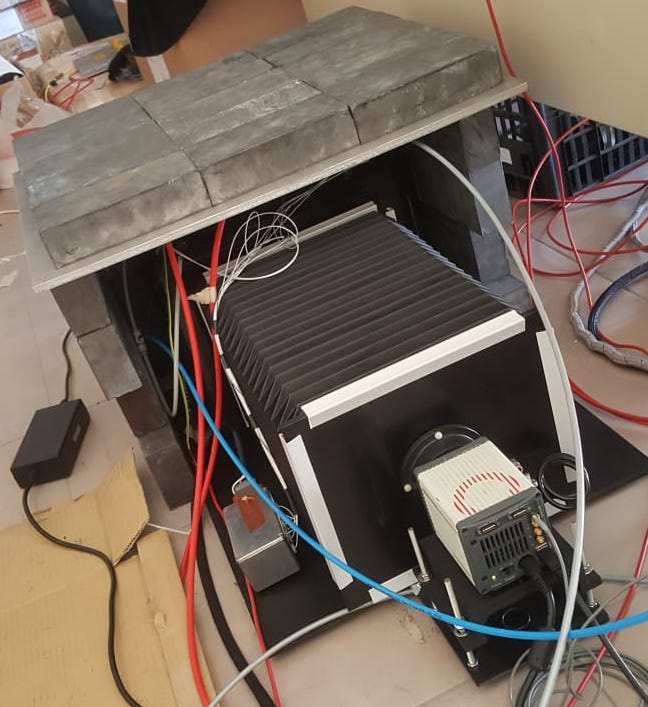
\includegraphics[width=0.45\linewidth]{LEMON-Shielded.jpg}
  	\caption{LEMOn with the lead shield of the  drift volume cage. The sCMOS camera (on the front) is looking at the GEMs through a blackened bellow.}
  	\label{fig:LemonShielded}
\end{figure}



A typical image frame obtained with a 30 ms exposure time of the sCMOS camera is shown in Fig.\ref{fig:typicalimage}. Several light spots are visible due to different ionization particles interacting in the gas.

\textcolor{red}{serve un'immagine senza il clustering e magari migliore di questa - forse per una pubblicazione occorre fare lo sfondo bianco ???}

 
\begin{figure}[ht]
	\centering
	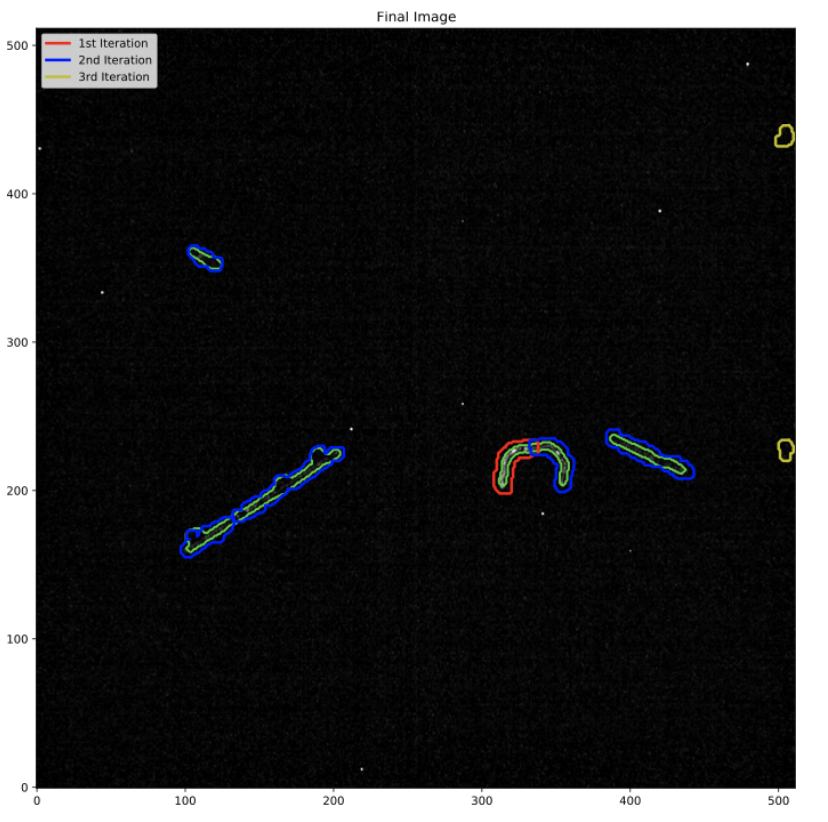
\includegraphics[width=0.45\linewidth]{typicalimage.png}
  	\caption{A picture taken with the sCMOS camera with a 30 ms exposure time. \textcolor{red}{ occorre aggiungere gli assi coordinati X e Y }}
  	\label{fig:typicalimage}
\end{figure}

LEMOn was operated in an overground location at Laboratori Nazionali di Frascati (LNF) with  a He-CF$_4$ (60/40) gas mixture, the triple GEM system set at a voltage across the GEM sides of xxx~V and an electric field between them of x.0 kV/cm - using a HV GEM power supply \cite{Corradi:2007df} ensuring stability and accurate monitoring of the bias currents. The gas mixture was kept at atmospheric pressure under continuous flow of about xxx cc/min and with the GEMs operated at $ x\times10^5$ gain. The typical photon yield for this  type of gas mixtures has been measured to be around  0.07 photons per avalanche electron.\cite{bib:jinst_orange1, bib:roby, bib:tesinatalia}

The field cage was powered by a CAEN N1570.\cite{CAENN1570} generating an electric field  of 0.6 kV/cm. 


\textcolor{red}{The ORCA Camera I/O has been configured in order to get a pre-trigger, that must occur 80~$\mu$s before the shutter, and to synchronize the PMT signal waveform acquired with an oscilloscope LeCroy 610Zi. Optics and exposure time (30~ms) were optimized to ensure the largest light collection and to avoid events due to the natural radioactivity. Between 100 and 300 images were typically acquired per run. }

A  5cm thick lead shielding was mounted around the LEMOn field cage to reduce the natural radioactivity background. From the measurements of the GEM current with and without the lead shielding a reduction of the total ionization in the sensitive gap, very likely due to external radioactivity of a factor 2 was estimated.

 An $Am$-$Be$ source with an activity of 3.5~$\times~$10$^3$~MBq was placed at a distance of 40~cm. This source isotropically emits:
 \begin{itemize}
     \item photons with an energy of 59~keV produced by $^{241}$Am;
     \item neutrons with a kinetic energy mainly in a range between 1 to 10 MeV due to the interaction of $\alpha$s emitted by the $^{241}$Am with the Be;
     \item photons with an energy of 4~MeV produced along with neutrons in the interacion between $\alpha$s and Be.
 \end{itemize}
 
The presence of lead shield around the sensitive volume absorbed almost completely the 59~keV photon component. A small faction of them reached the gas trough small slits accidentally present between the bricks.
 

 \section{Cluster pattern recognition}
 

Define basic 
 \section{Cluster observables}
 
 Define  (projected) length $l$, light $L$, energy $E$ (light after calibration), density of light $\delta$ (and then $\frac{dE}{dl}$ after calibration but projected that's why I am using $dl$ !), slimness $S$
 
 Describe here briefly the $E$ calibration ? saturation effect removal ? 
 
 \section{Nuclear recoil identification results}
 
 During the data-taking xxx frames were recorded in absence of any external source ({\it no-source} sample). In these frames the interaction of ultra-relativistic cosmic ray particles (mostly muons) are clearly visible  as  very long cluster. Internal radioactivity of the LEMOn materials  also contribute several smaller size cluster.  It is then possible to define a pure sample of cosmic ray tracks by requiring $L$ > 13 cm and $S$ < 0.1  \textcolor{red}{che altro manca? }. The cosmic ray cluster identified with this selection show small values of  $\delta$ $\sim $ 5 well compatible with the small specific ionization of ultra-relativistic particles. 
 In Fig.\ref{fig:cosmics} we show the distribution of the observed $\frac{dE}{dl}$ for the no-source sample and for the Am-Be samples. The broadening of the distribution is mainly due to the specific energy loss fluctuation in the gas mixture of the cosmic ray particles.   Its mean value corrected for the effect of the angular distribution of the cosmic rays is   xx keV/cm that is in good agreement with the Garfield prediction of 2.3 keV/cm.  The angle with the horizontal axis is evaluated by  measuring the distance between \textcolor{red}{EAM spiega come hai fatto}. In Fig.\ref{fig:cosmics} the distribution   of the  angle of the cosmic ray cluster in the no-source sample is shown.
 
 
 \begin{figure}[ht]
	\centering
	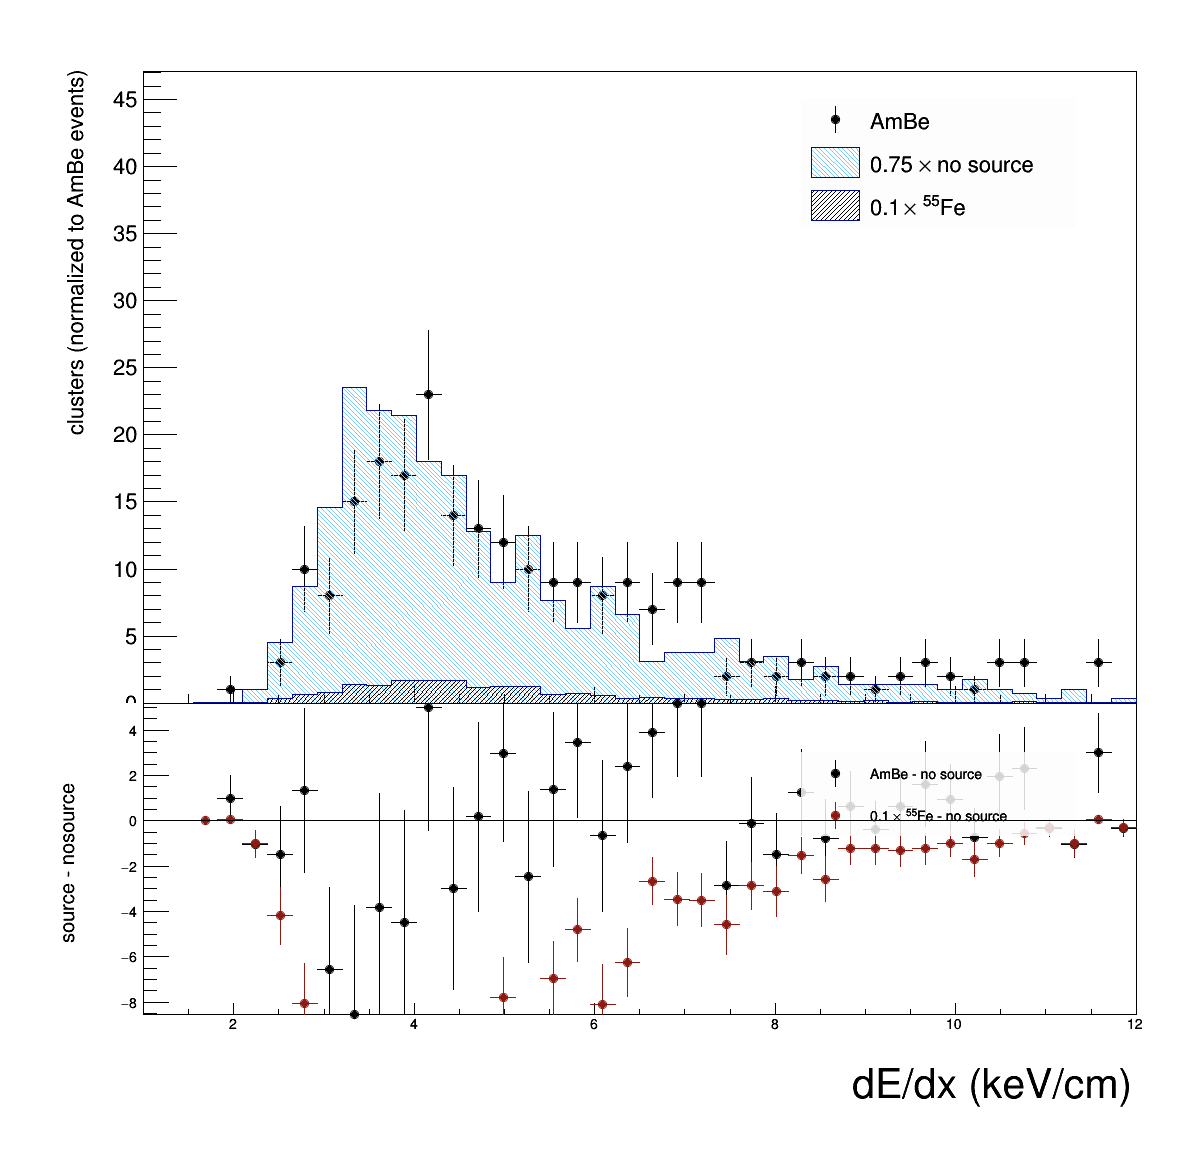
\includegraphics[width=0.45\linewidth]{dEdx_cosmics.png}
	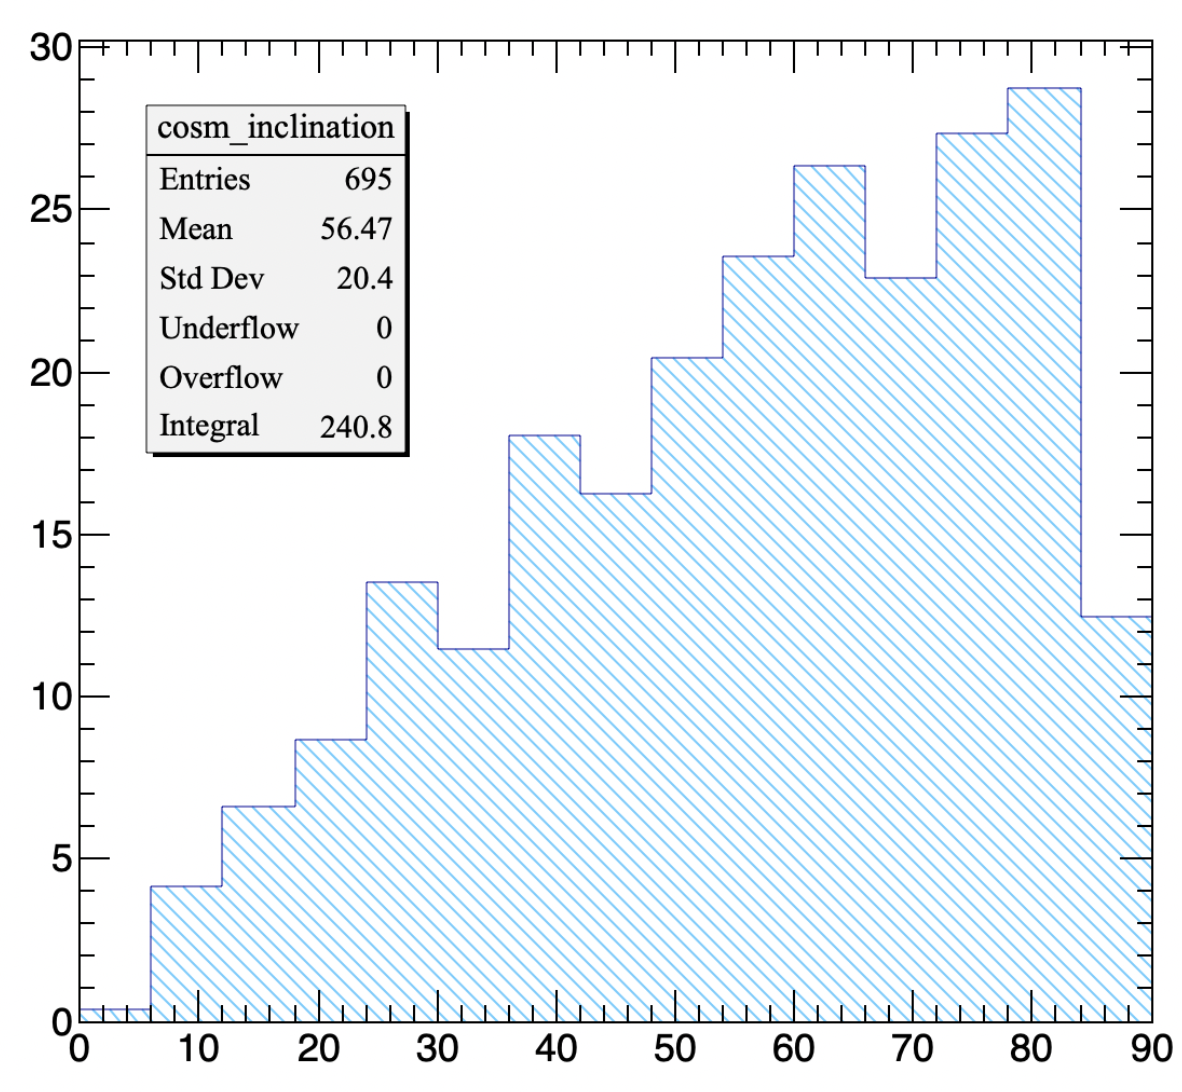
\includegraphics[width=0.45\linewidth]{cosmic_angle.png}
  	\caption{Left: Distributions of reconstructed energy release per centimetre for cosmic rays. Right: Distributions of reconstructed angles for cosmic rays. }
  	\label{fig:cosmics}
\end{figure}
\textcolor{red}{Non farei vedere il Ferro in questa figura. Inoltre il plot delle differenza deve essere fatto su scala diversa. }

 
 \section{Conclusion and Outlook}
 
 


\begin{figure}[ht]
	\centering
	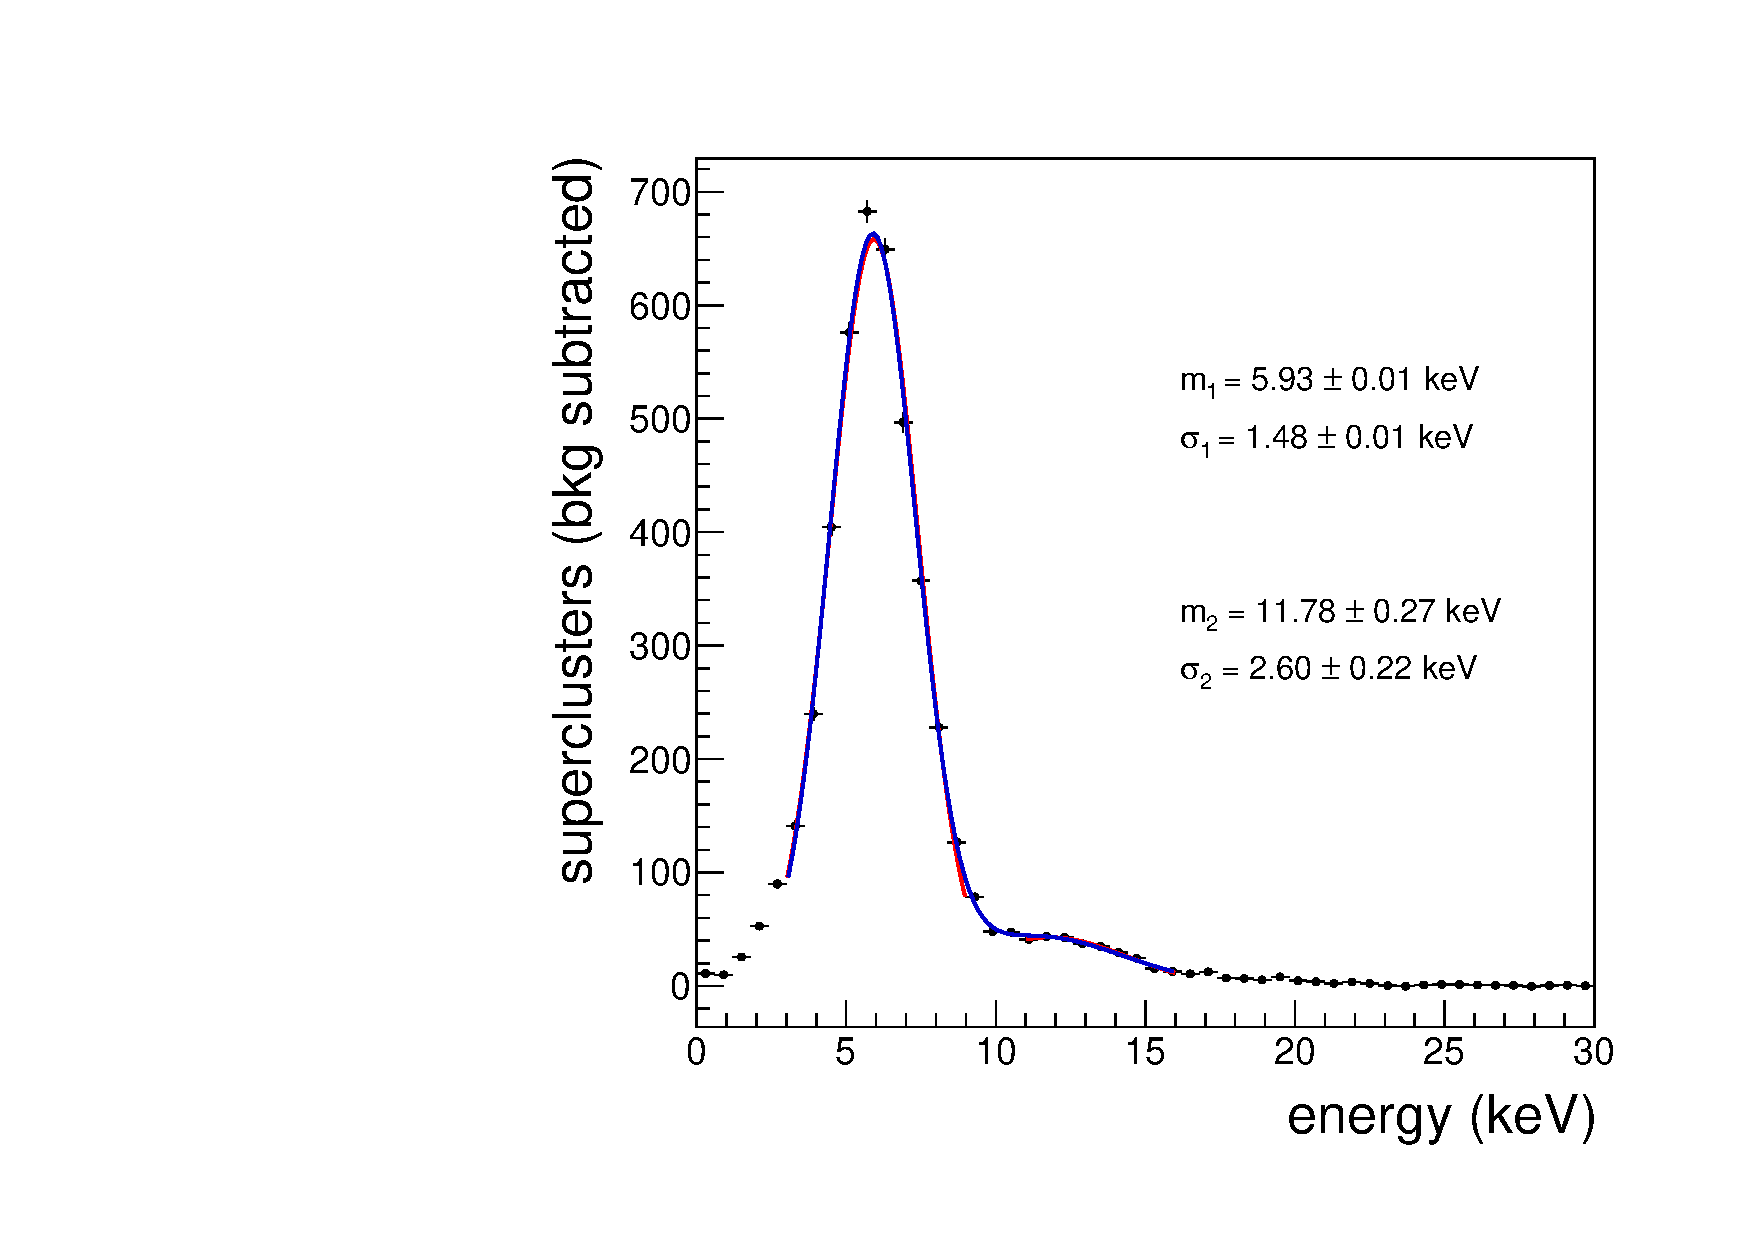
\includegraphics[width=0.45\linewidth]{fe_diff_simplefit.pdf}
	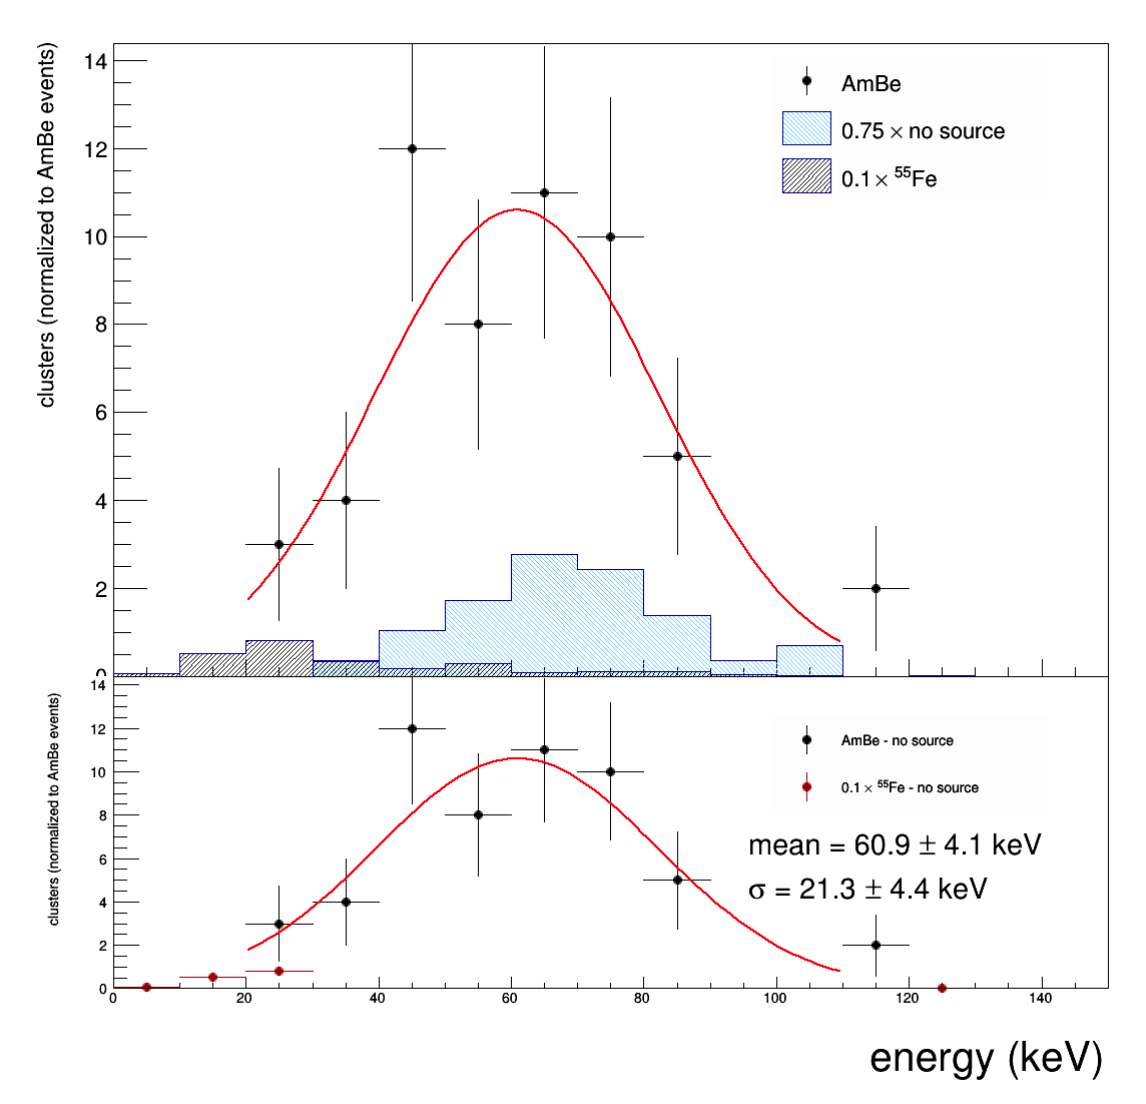
\includegraphics[width=0.45\linewidth]{spectrum_59keV.png}
  	\caption{Left: Spectrum of energy of the clusters reconstructed as produced by interactions of 5.9~keV photons in gas. Right: Spectrum of energy of the clusters reconstructed as produced by interactions of 59~keV photons in gas.}
  	\label{fig:55Fe&59keV}
\end{figure}

\begin{figure}[ht]
	\centering
	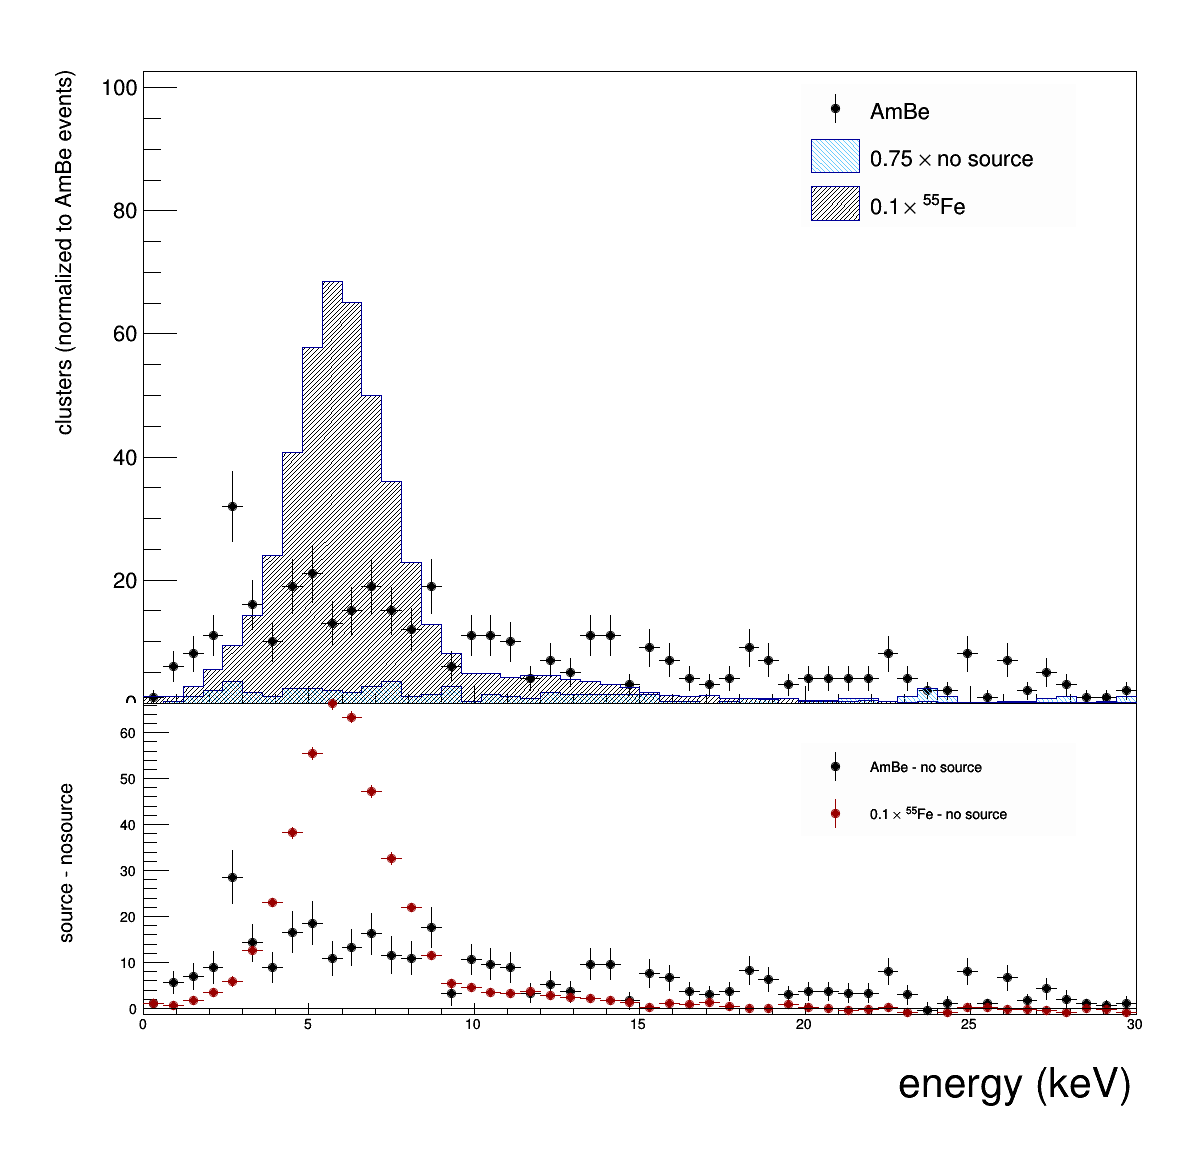
\includegraphics[width=0.45\linewidth]{energy_spectrum.png}
	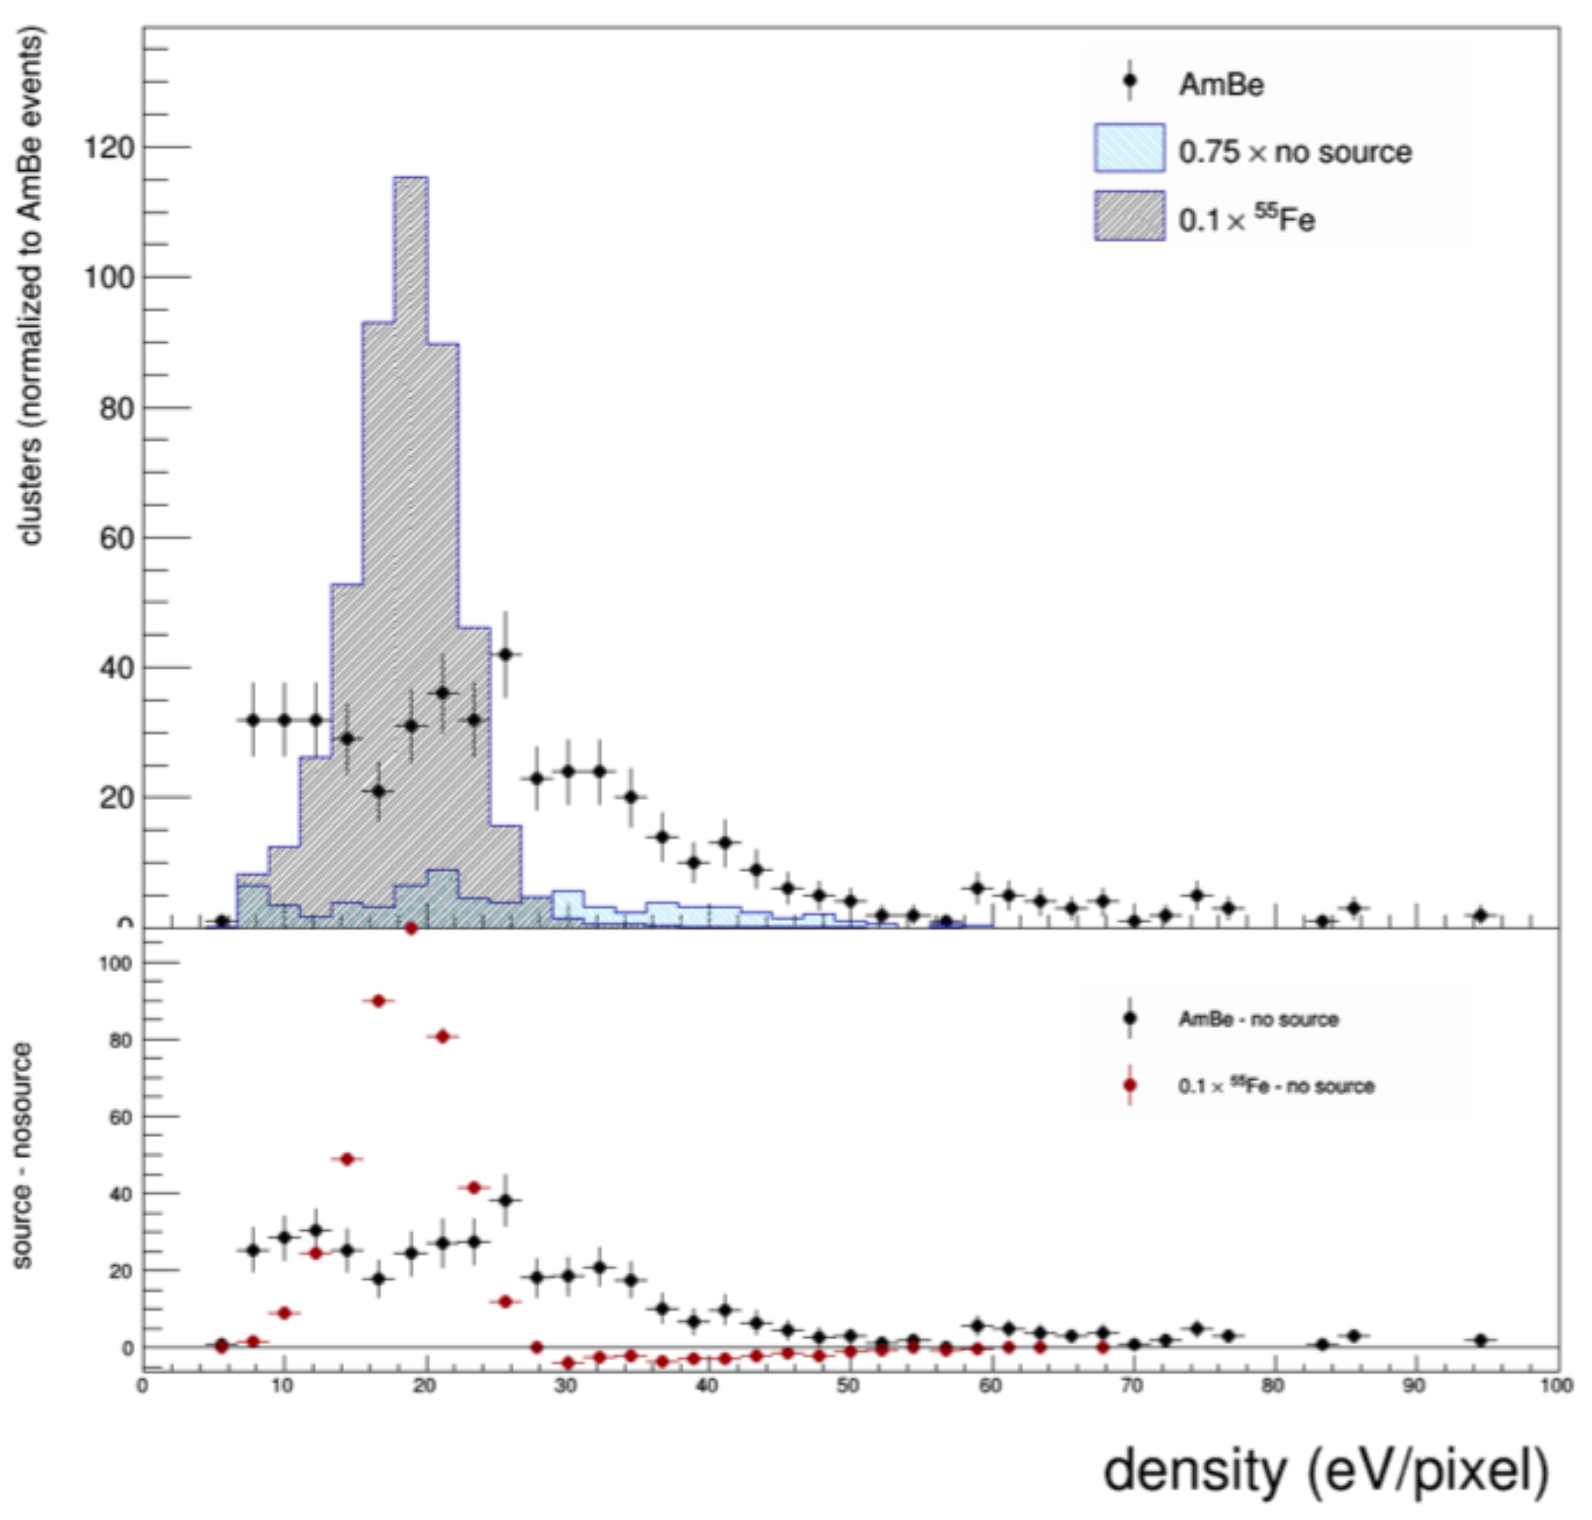
\includegraphics[width=0.45\linewidth]{density_spectrum.png}
  	\caption{Spectra of energy (left) and energy density (right) of the clusters reconstructed in three different run types after the preliminary cuts.}
  	\label{fig:ene&dens}
\end{figure}

\begin{figure}[ht]
	\centering
	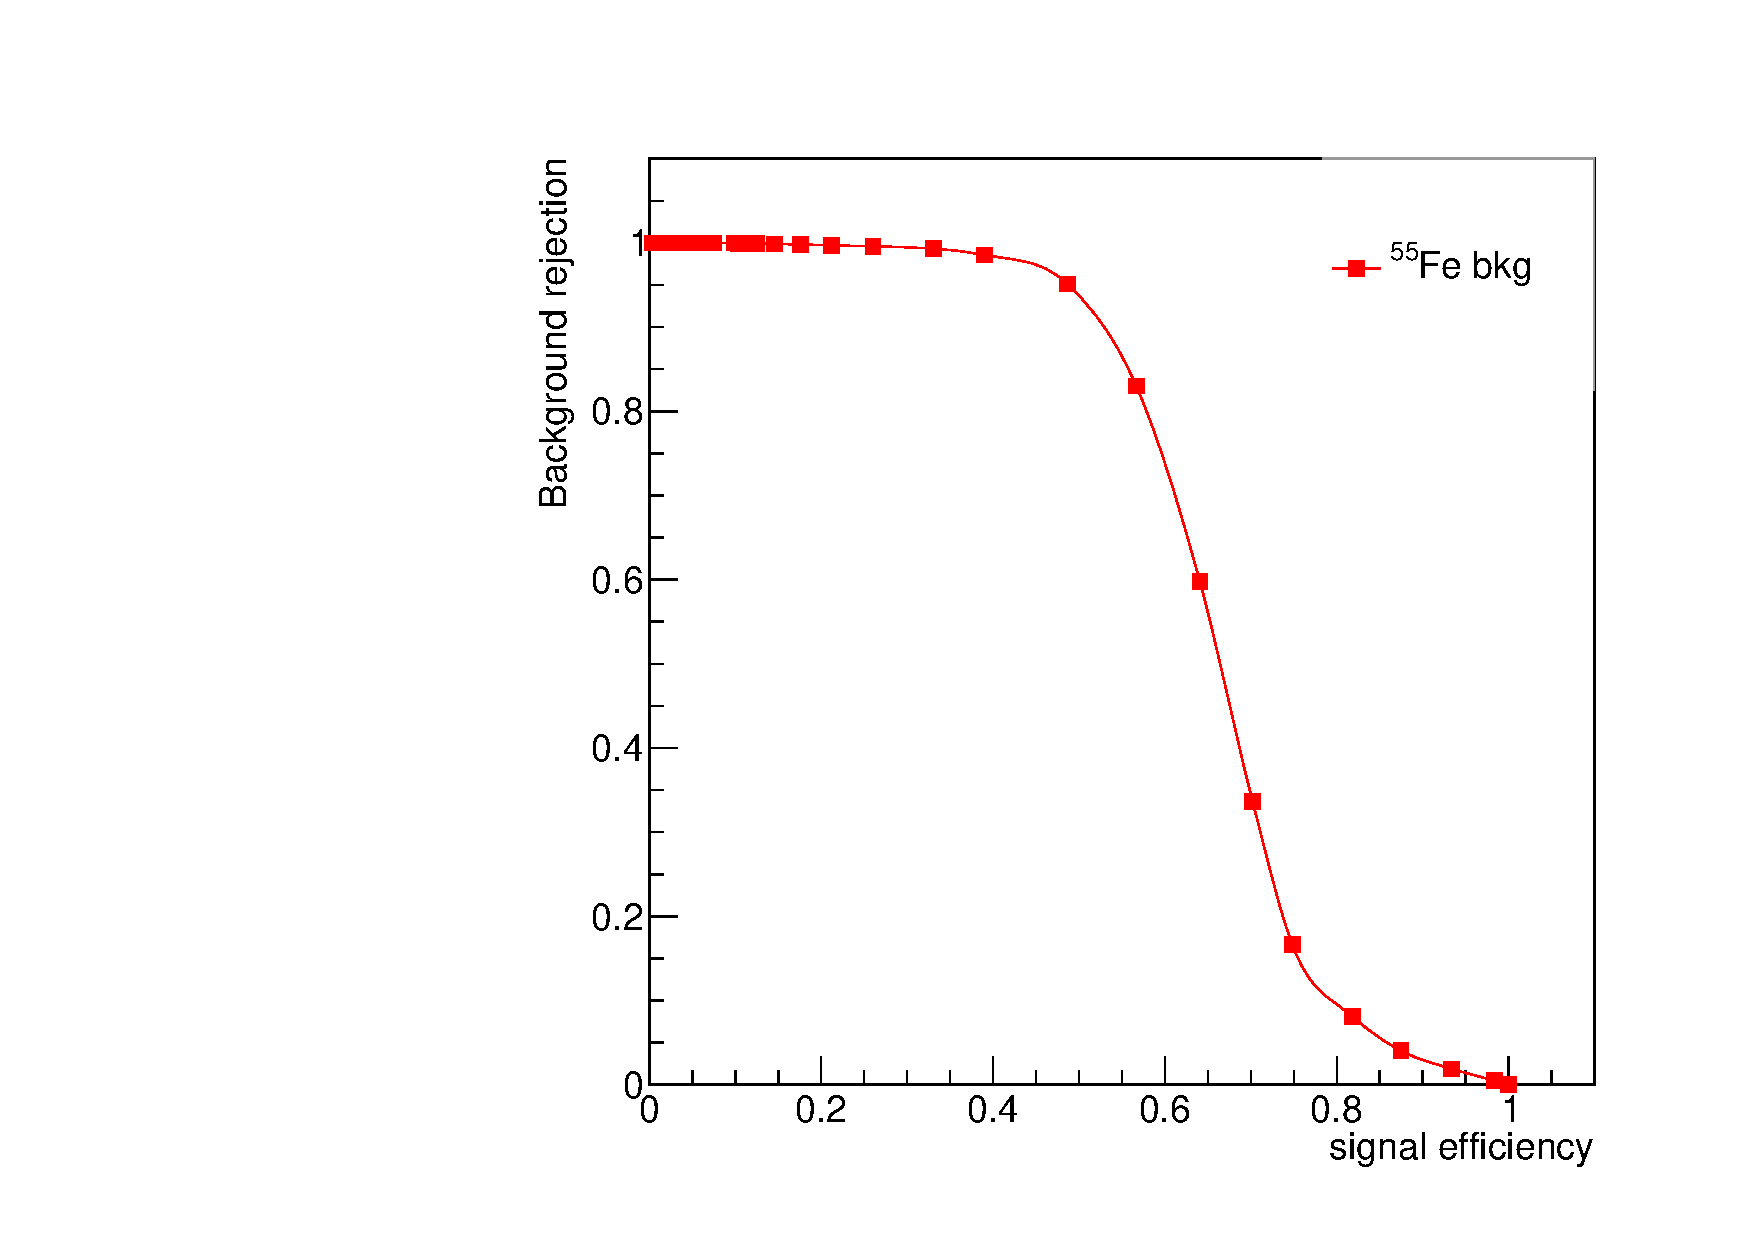
\includegraphics[width=0.50\linewidth]{density_roc.pdf}
  	\caption{Electron Recoil (ER) signal rejection as a function of the Nuclear Recoil signal detection efficiency.}
  	\label{fig:roc}
\end{figure}
\textcolor{red}{per un paio di punti scriverei vicino il taglio density > ...}

\begin{figure}[ht]
	\centering
	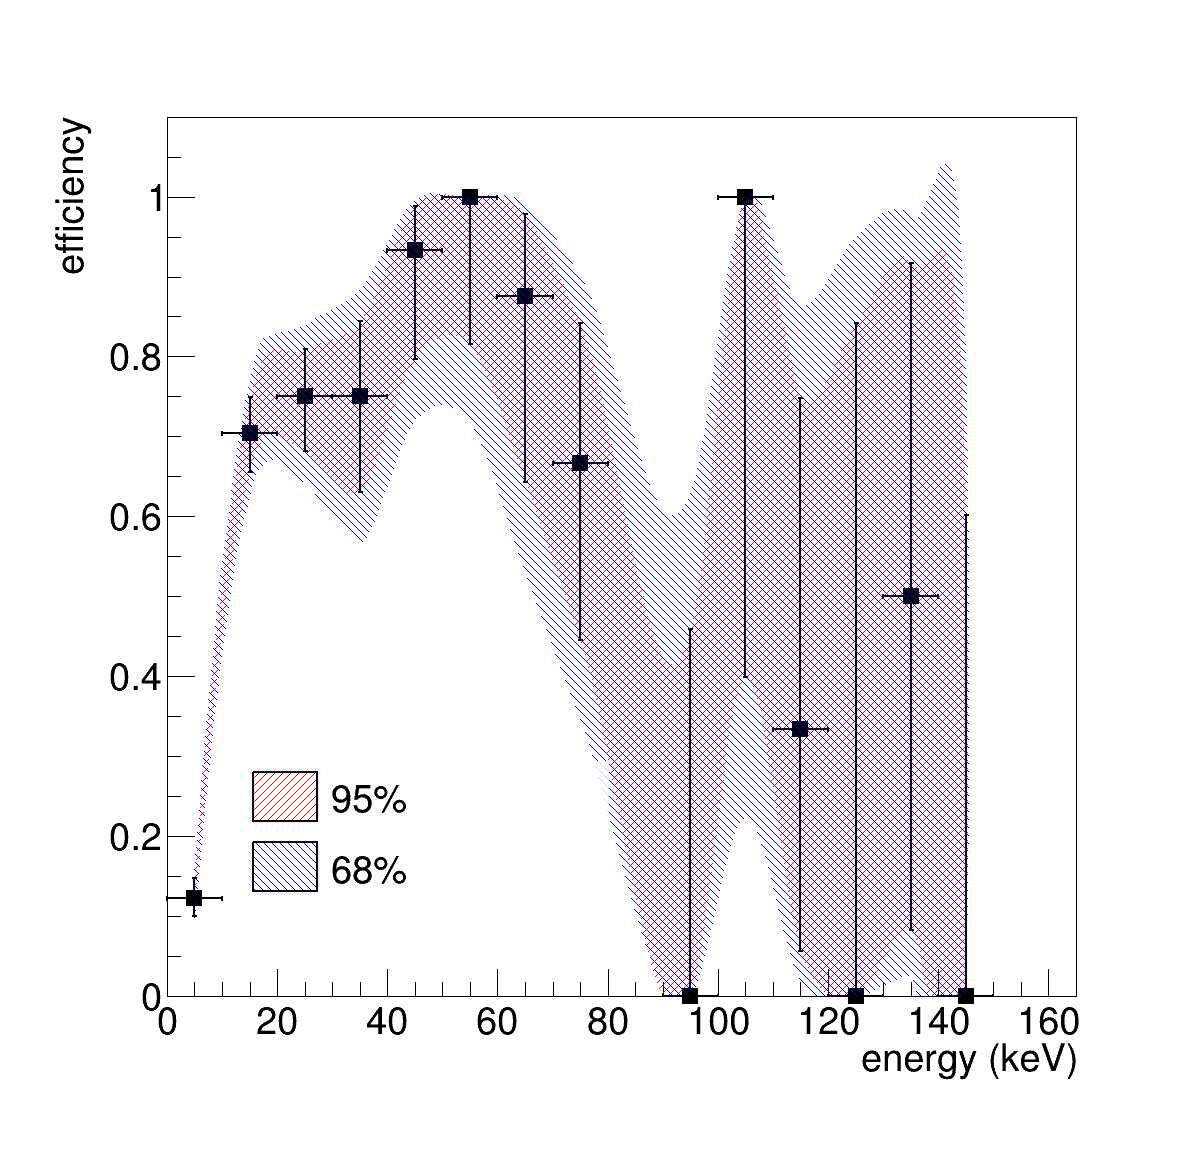
\includegraphics[width=0.45\linewidth]{effS.png}	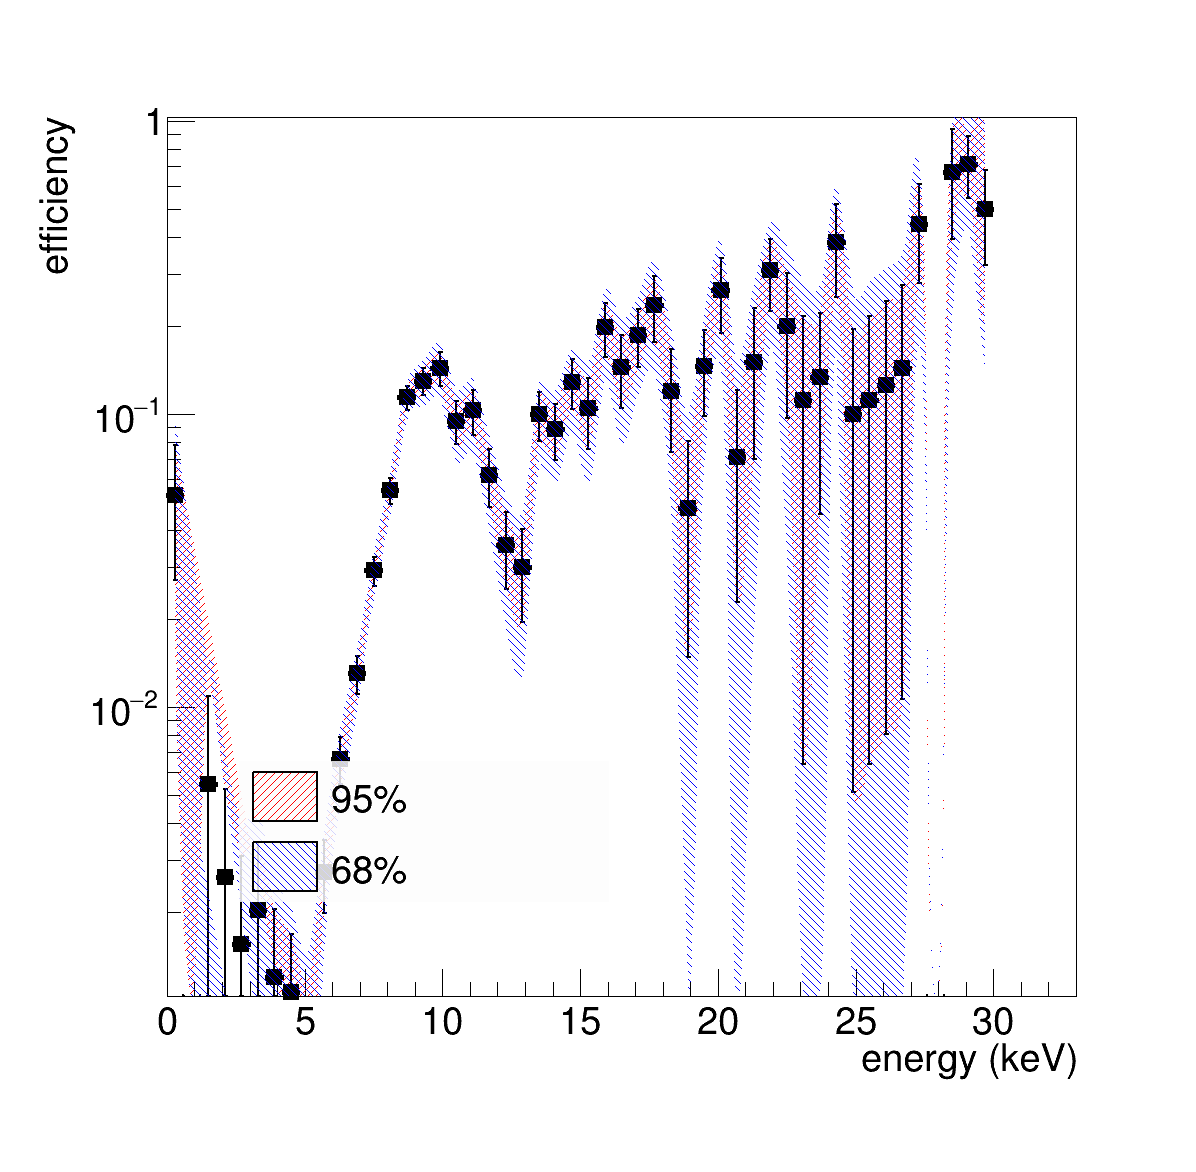
\includegraphics[width=0.45\linewidth]{effB.png}
  	\caption{Detection efficiency of Nuclear Recoil (NR) signals (left) and Electron Recoil (ER) signals (right) as a function of their reconstructed energy.}
  	\label{fig:effB}
\end{figure}


\begin{figure}[ht]
	\centering
	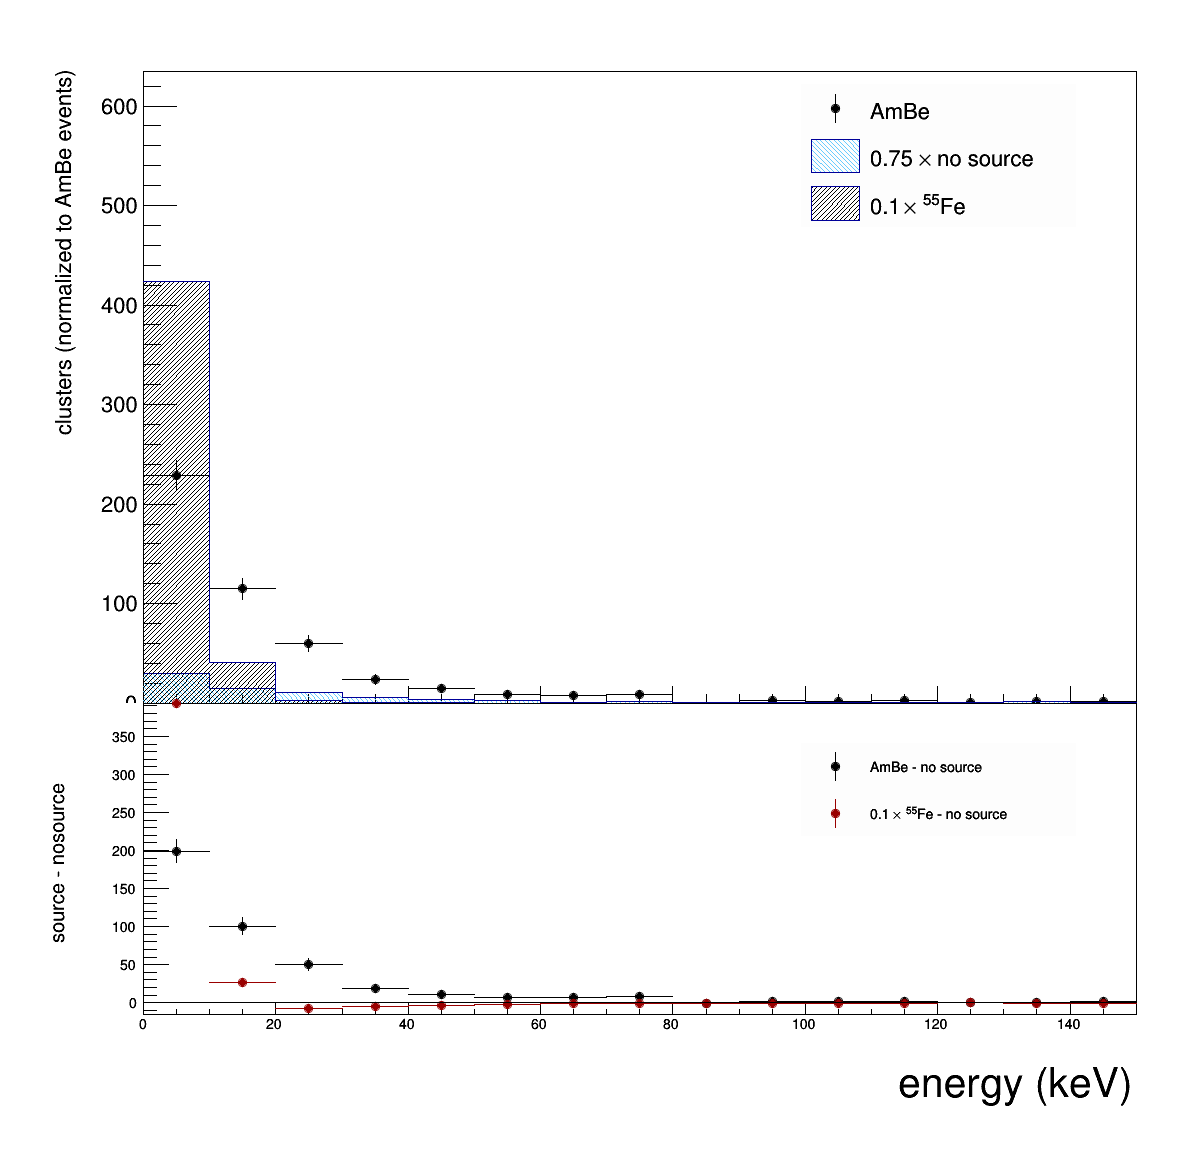
\includegraphics[width=0.45\linewidth]{energyExt.png}
	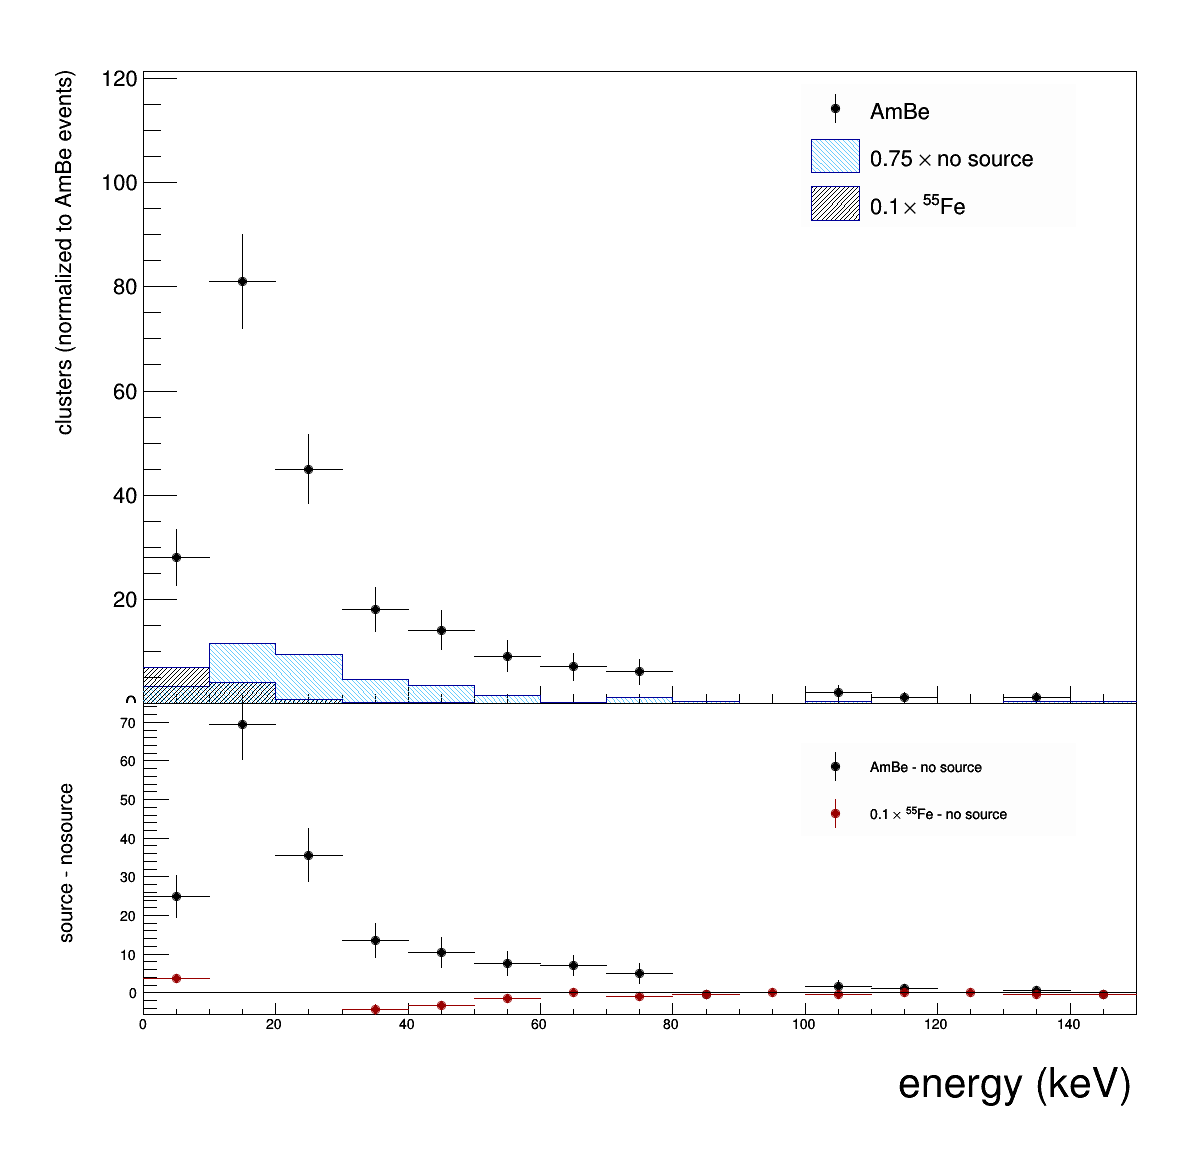
\includegraphics[width=0.45\linewidth]{energyExt_cut.png}
  	\caption{Spectra of energy of the clusters reconstructed in three different run types before (left) and after (right) cuts on energy densities.}
  	\label{fig:energy}
\end{figure}
\textcolor{red}{vogliamo provare a dimizzera la bin widt per gli spettri in energia?}
\begin{figure}[ht]
	\centering
	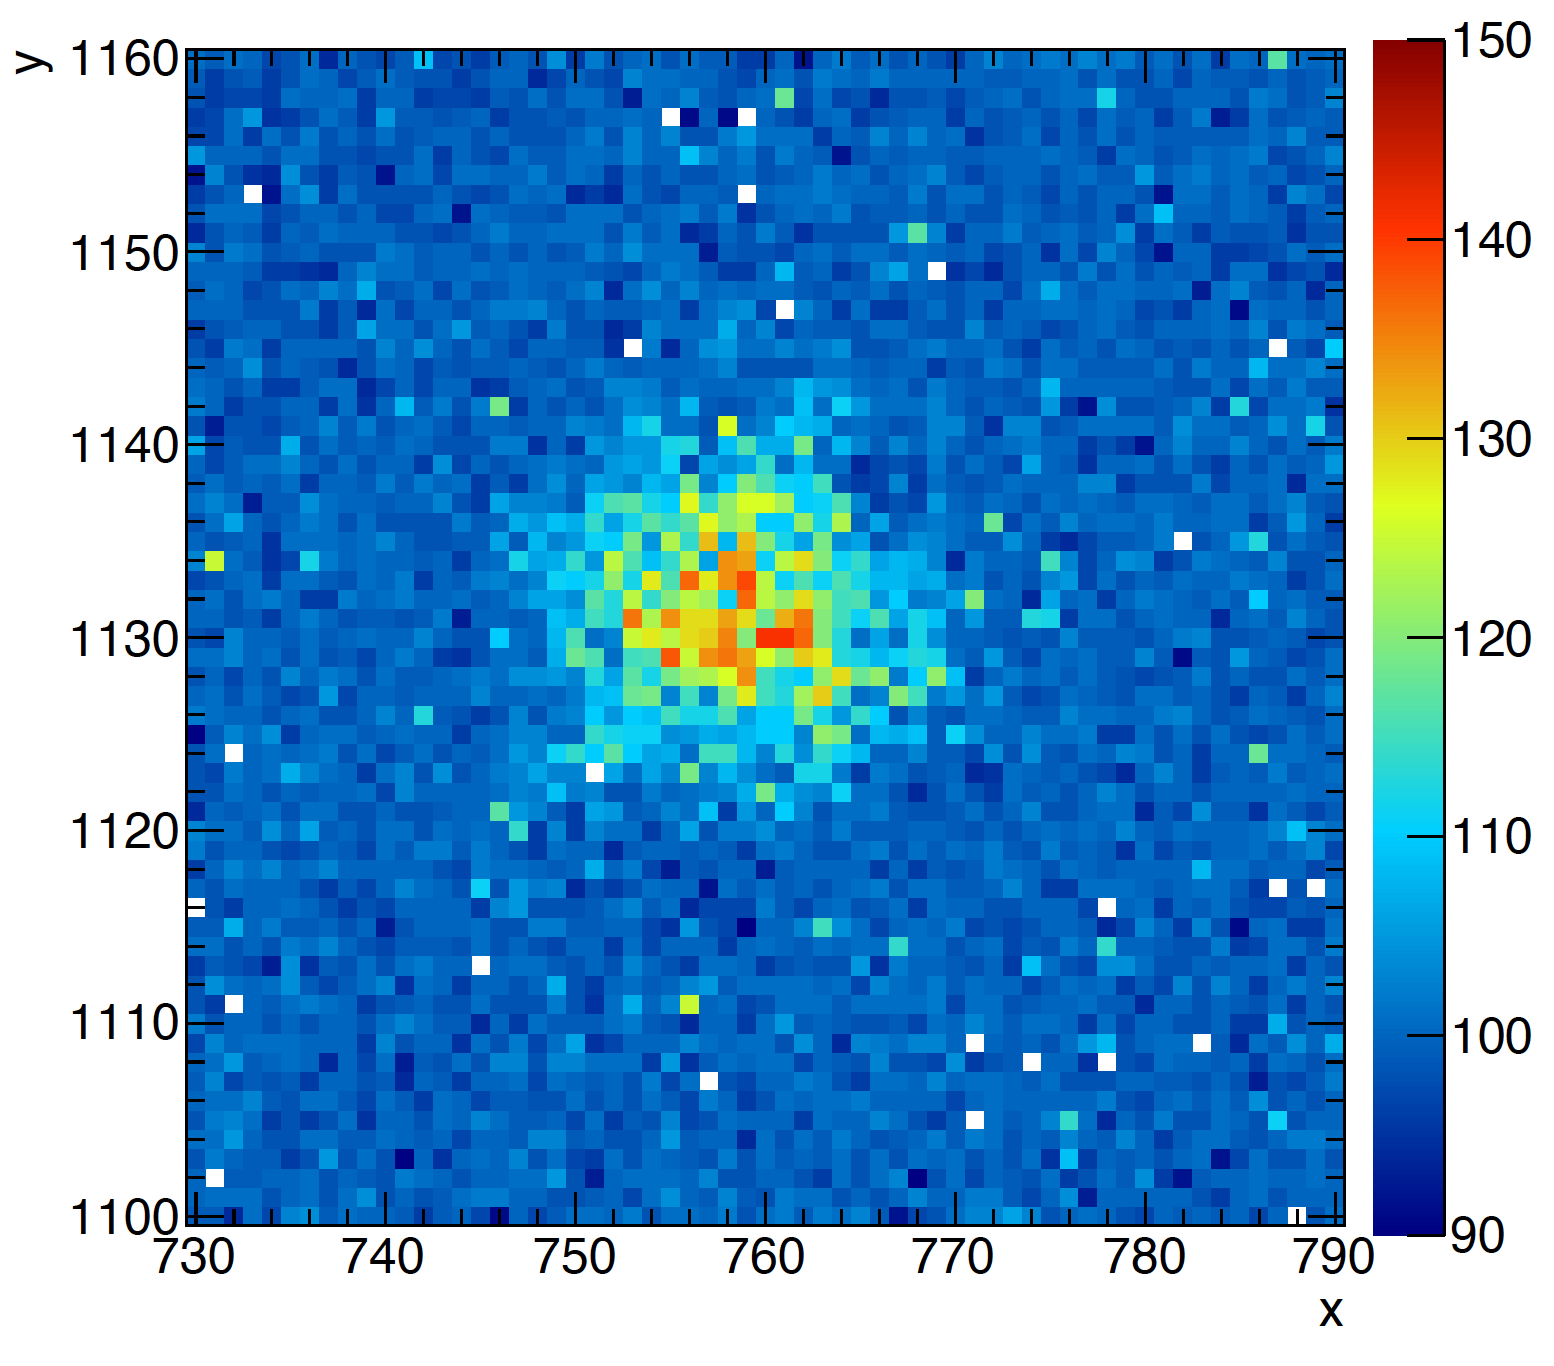
\includegraphics[width=0.50\linewidth]{granchio.png}
  	\caption{Example of a signal reconstructed as a Nuclear Recoil (NR) with an energy of 9~keV.}
  	\label{fig:granchio}
\end{figure}

\textcolor{red}{non farei vedere electron recoil che non ha senso in funzione dell'energia con questo campione }


\bibliography{mybiblio}{}
\bibliographystyle{plain}

\end{document}

